\documentclass[aspectratio=169,xcolor=table]{beamer}
%aspcetratio >> 1610 169 149 54 43 32
%The themes:
\usetheme[style=classic]{mharvellous}
%\usetheme[style=dark]{mharvellous}
%\usetheme[style=mracula]{mharvellous}
% \usetheme[style=default]{mharvellous}
%*--------------------------------------------------
%\usepackage{helvet}
%*--------------------------------------------------
\usepackage{bibunits}  
%\setbeamertemplate{bibliography item}{[\theenumiv]}
\setbeamertemplate{bibliography item}{\insertbiblabel}
\defaultbibliography{bibliography}
%\defaultbibliographystyle{IEEEtran}
%\defaultbibliographystyle{amsalpha}
\defaultbibliographystyle{abntex2-alf}
%\bibliography{bibliography}
%\usepackage[backend=biber,style=alphabetic,citestyle=authoryear]{biblatex}
% \addbibresource{bibliography.bib}
%\usepackage{natbib}
\usepackage{bibentry}
%*--------------------------------------------------
\usepackage{lipsum}
\usepackage{epigraph}
\usepackage{graphicx}
\usepackage{multirow}
%\usepackage{enumitem}
\usepackage{array}
%\usepackage{multimedia}
\usepackage{media9}
%\usepackage{pdfpc-movie}
\usepackage{circledsteps}
\usepackage{listings}
\usepackage[normalem]{ulem}
%\usepackage{Sweave}
%\usepackage{xkeyval}
%\usepackage{palatino}
%\usepackage{pgfpages}
\usepackage{float}
%*--------------------------------------------------
\usepackage[timeinterval=1]{tdclock}
%\usepackage[font=Times,timeinterval=1, timeduration=200,resetatpages=all]{tdclock}
%\usepackage[font=Times,timeinterval=10, timeduration=2.0, timedeath=0, fillcolorwarningsecond=white!60!yellow,timewarningfirst=50,timewarningsecond=80,resetatpages=2]{tdclock}
%*--------------------------------------------------
\usepackage{url}
\usepackage{tabularx,booktabs}
\usepackage{threeparttable}
\usepackage[absolute, overlay]{textpos}
%*--------------------------------------------------
\usepackage{framed, color}
\usepackage[tikz]{bclogo}
\usepackage{spot}
\setspotlightcolor{red!50}
% %\setspotlightstyle{star, fill=red!50}
% %\setspotlightstyle{star points=7}
\usepackage{color,soul}
%\usepackage{xcolor}
\usepackage{tcolorbox}
\usepackage{xcolor}
\usepackage[export]{adjustbox}
\usepackage{verbatim}
\usetikzlibrary{trees,shapes,arrows}
\usepackage{fancyvrb}
\usepackage{float}
%*--------------------------------------------------
\usepackage{amsmath}
\usepackage{xfrac}
\usepackage{units}
\usepackage{ulem}
%*-------------------------------------------------------------------------------
%\newcolumntype{C}[1]{>{\centering\arraybackslash}m{#1}}
\newcolumntype{L}[1]{>{\raggedright\let\newline\\\arraybackslash\hspace{0pt}}m{#1}}
\newcolumntype{C}[1]{>{\centering\let\newline\\\arraybackslash\hspace{0pt}}m{#1}}
\newcolumntype{R}[1]{>{\raggedleft\let\newline\\\arraybackslash\hspace{0pt}}m{#1}}
%*-------------------------------------------------------------------------------
%\pgfpagesuselayout{2 on 1}[a4paper,border shrink=5mm]
%\setbeamertemplate{note page}[plain]
%\setbeameroption{show notes on second screen=bottom}
%*-------------------------------------------------------------------------------
\setbeameroption{hide notes}
%\setbeameroption{show only notes}
%\setbeameroption{show notes on second screen=right}
\setbeamertemplate{note page}{\pagecolor{yellow!5}\insertnote}
%*-------------------------------------------------------------------------------

%*-------------------------------------------------------------------------------
\title              {OPEN Manipulator}
\subtitle           {Project Follow Up}
\author             {Anderson Lima \& Juliana Santana}
\email              {anderson.farias@fbter.org.br \& juliana.maria@fbter.org.br}
\advisor            {Orientador: Marco A. dos Reis}
\institute          {Robótica e Sistemas Autônomos, Senai Cimatec}
\date               {Fevereiro de 2022}
% \ulogo        		{Template/logosenaicimatecnegativo}
% \ulogof             {Template/logosenaicimatec2020}
% \ulogoo        		{Template/rosa-logo}
% \ulistelement    	{Template/bullet-white}

%*-------------------------------------------------------------------------------
\graphicspath{{Source/pictures/}}
%*-------------------------------------------------------------------------------
\totalNoSlidesDisabled % To turn off the total number of slides in the footer. Comment this if you want the total number of slides in the footer
%*-------------------------------------------------------------------------------
 \begin{document}
%*----------- COVER -------------------------------------------------------------
  \begin{frame}[t,plain]
%*----------- sound--------------------------------
    \includemedia[
        %width=1ex,
        %height=1ex,
        %activate=pageopen, 
        activate=onclick,
        deactivate=onclick,
        %passcontext,
        transparent,
        addresource=./Source/sounds/hip-hop.mp3,
        flashvars={
                    source=./Source/sounds/hip-hop.mp3
                    %&autoPlay=true
                    &autoRewind=true
                    &Play=2s
                    &repeat=always
                    %&Loop=true
        }
    ]
    {}{VPlayer.swf}
%*----------- start-page--------------------------
     \titlepage
    %*----------- notes-------------------------------
    \note[item]{Notes can help you to remember important information. Turn on the notes option.}
\end{frame}
%-
%*----------- SECTIONS ----------------------------------------------------------
%*----------- SLIDE -------------------------------------------------------------
 %*----------- SLIDE (IMAGEM DO PROJETO) -------------------------------------------------------------
 \begin{frame}[t]{OPEN Manipulator Pro}
    \begin{figure}
        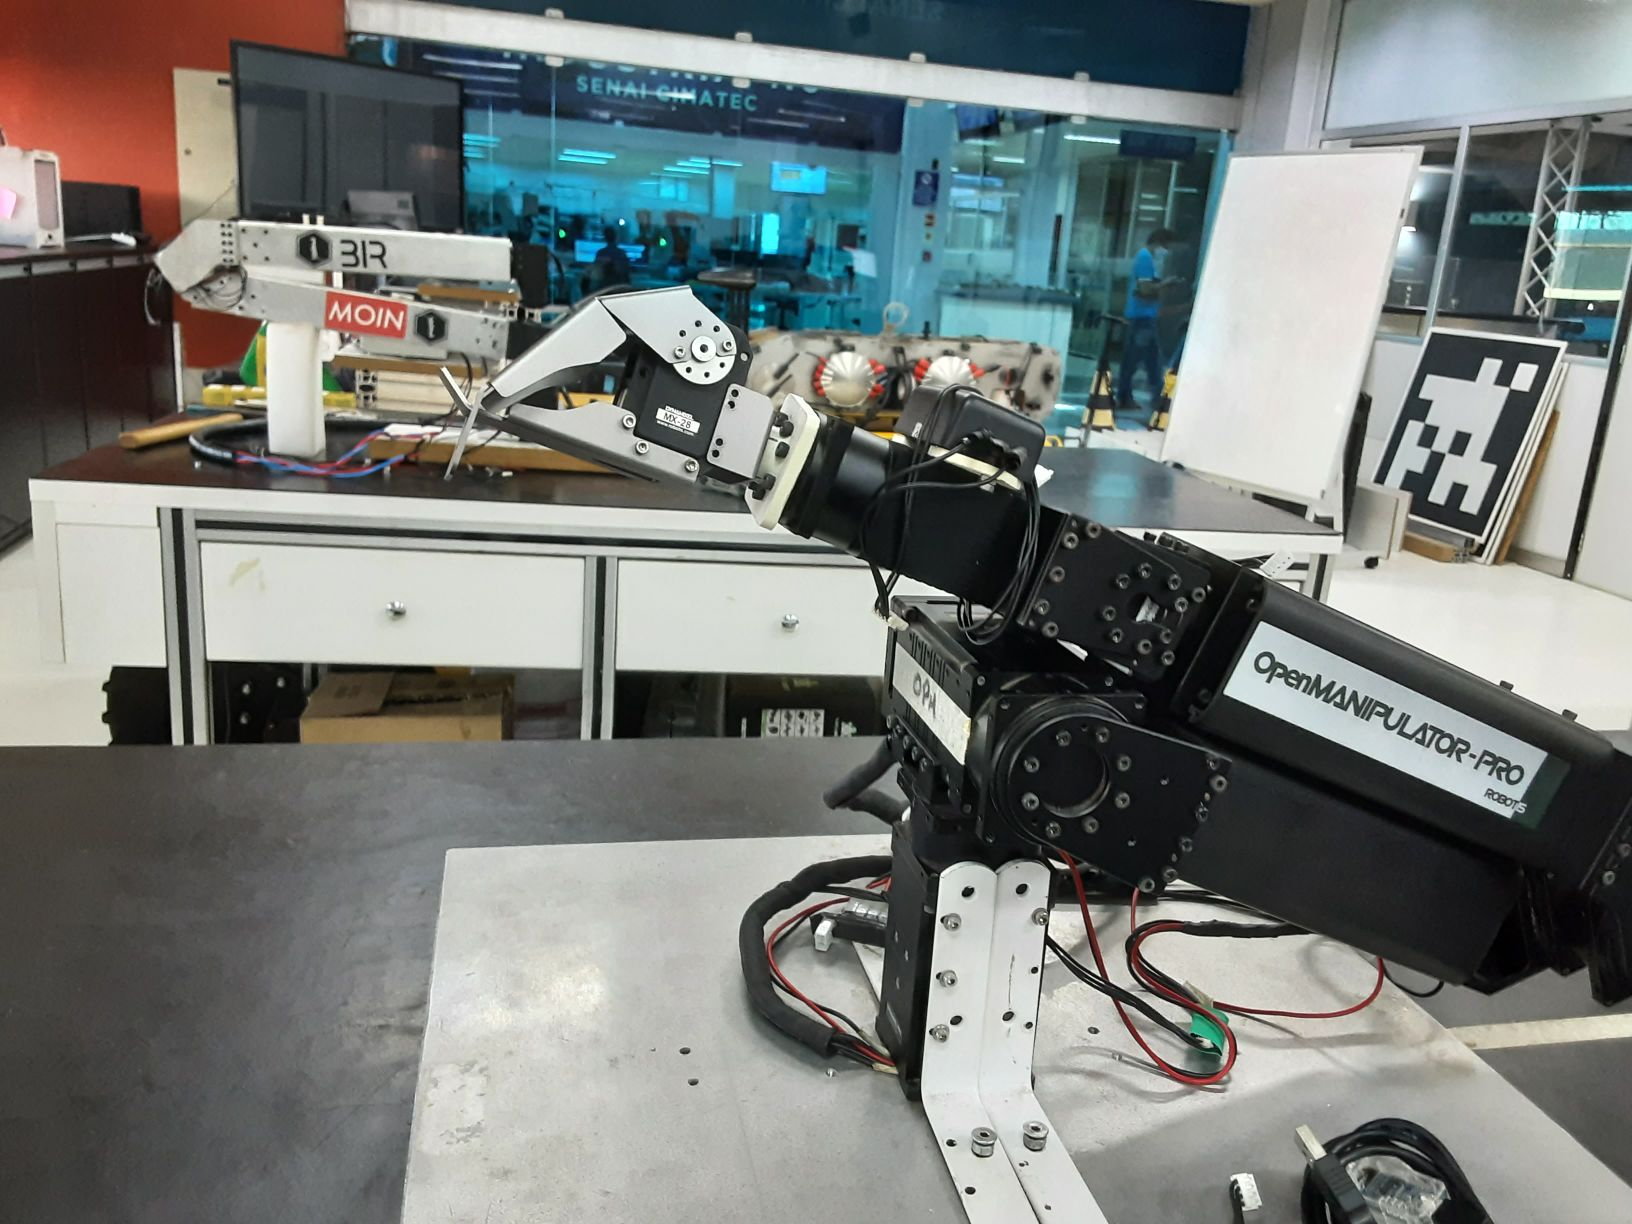
\includegraphics[width=0.60\textwidth]{manipulador.jpg}
        %\caption{.}
    \end{figure}
\end{frame}
 %*----------- SLIDE (IMAGEM DO PROJETO) -------------------------------------------------------------
 \begin{frame}[t]{Andamento do projeto}
    \begin{figure}
        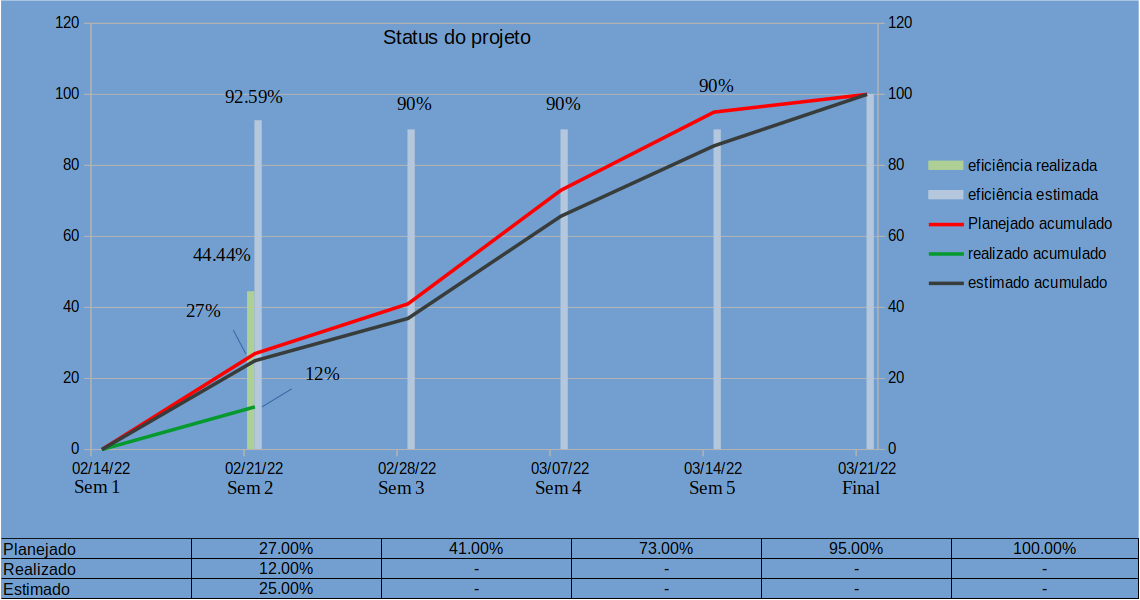
\includegraphics[width=0.85\textwidth]{planejamento-follow-up-16-02-2022.png}
        %\caption{.}
    \end{figure}
\end{frame}

%-------------------------------------------------------------
\begin{frame}[c]{Andamento do projeto}
    \begin{table}[ht!]
    \centering
        \caption{PERCENTUAL DE CONCLUSÃO}
        \begin{tabular}{|c|c|c|c|c|} \hline
            \textbf{Estado Anterior}&\textbf{Estado Atual}&\textbf{Eficiência}\\\hline
            0\% &12\% &44.44\% \\ \hline
        \end{tabular}
    \end{table}
    \begin{table}[ht!]
        %\centering
            \caption{ATIVIDADES REALIZADAS}
            \begin{tabular}{|c|c|c|c|} \hline
                \textbf{Atividade}&\textbf{Porcentagem}&\textbf{Atividade}&\textbf{Porcentagem}\\\hline
                Verificar documentações &60\% &   WBS        &80\% \\ \hline
                Customer Requirements   &0\%  &   PBS        &80  \% \\ \hline
                Arquitetura Geral       &50\% &   Simulação  &0\%  \\ \hline

            \end{tabular}
        \end{table}
%*----------- notes
    \note[item]{Notes can help you to remember important information. Turn on the notes option.}
\end{frame}
%-
%*----------- SLIDE -------------------------------------------------------------
\begin{frame}[t]{WBS}

    \begin{figure}
        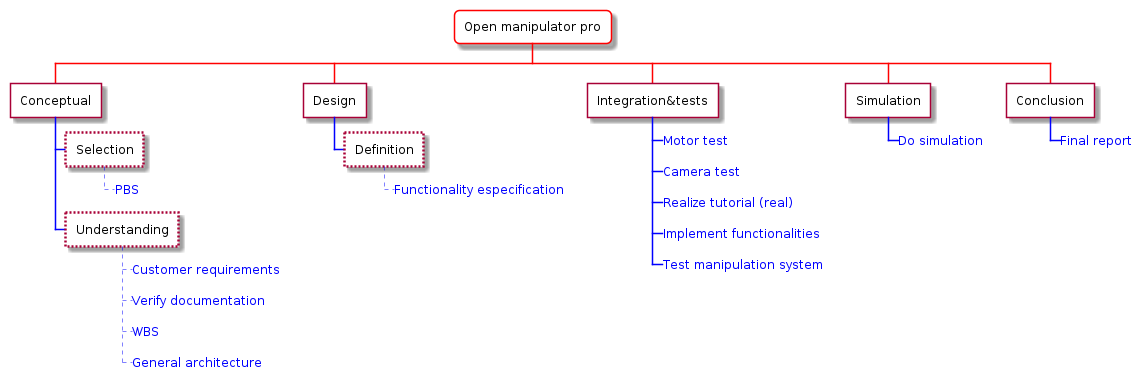
\includegraphics[width=1\textwidth]{wbs.png}
         %\caption{.}
     \end{figure}
 %*----------- notes
 %    \note[item]{Notes can help you to remember important information. Turn on the notes option.}
 \end{frame}
 %-
 %*----------- SLIDE -------------------------------------------------------------
 \begin{frame}[t]{PBS}
 
     \begin{figure}
         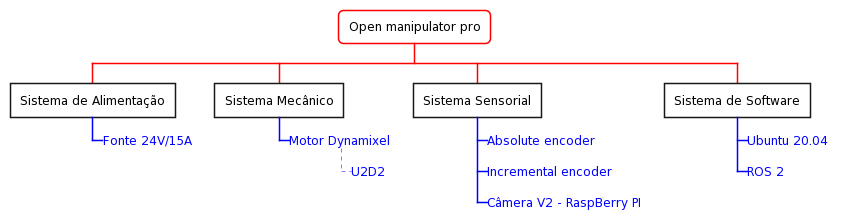
\includegraphics[width=1
         \textwidth]{PBS.png}
         %\caption{.}
     \end{figure}
 %*----------- notes
     \note[item]{Notes can help you to remember important information. Turn on the notes option.}
 \end{frame}
 %--------------------------------------------------------------------------------
  %*----------- SLIDE -------------------------------------------------------------
  \begin{frame}[t]{Arquitetura Geral}
 
    \begin{figure}
        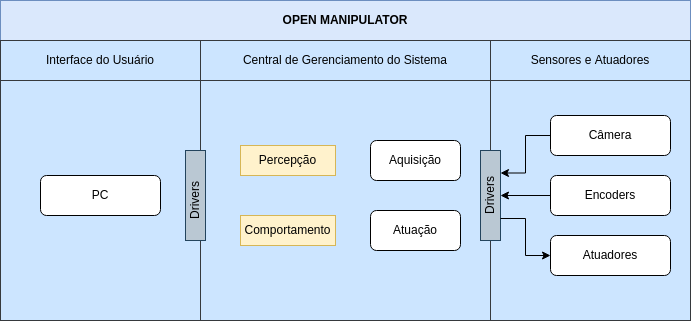
\includegraphics[width=0.90
        \textwidth]{arquitetura-geral.png}
        %\caption{.}
    \end{figure}
%*----------- notes
    \note[item]{Notes can help you to remember important information. Turn on the notes option.}
\end{frame}
%--------------------------------------------------------------------------------
%-
%*----------- SLIDE-BACKUP ------------------------------------------------------
% \backupbegin
% %
% \begin{frame}{Backup}
%     Test
% %*----------- notes-------------------------------
% \note{Notes can help you to remember important information. Turn on the notes option.}
% \end{frame}
% %-
% \backupend
% %-
%*----------- QUESTIONS ---------------------------------------------------------
\begin{frame}[c,plain]
    \lastpage{
        \begin{center}   
            {\usebeamerfont{title} Questions?}\\[3ex] 
            %\hspace{1.5cm} 
            anderson.farias@fbter.org.br juliana.maria@fbter.org.br
        \end{center}
    }

    %*----------- notes---------------------------------
    \note[item]{Notes can help you to remember important information. Turn on the notes option.}
\end{frame}
%*-------------------------------------------------------------------------------
\end{document}